\section{Energy Harvesting Techniques} \label{sec:eh}
% how to relate this to my research

Although all kinds of energy harvesters can extract energy from ambient sources, they have various output characteristics in terms of the amount and dynamics of the harvested power depending on the ambient energy conditions and energy harvesting techniques. 
To select an energy harvester for powering sensor nodes, one important concern is whether the supply power level matches the consumption of the load~\cite{shaikh2016energy}. 
For one certain type of energy harvesters, the harvested power can be scaled by the power density of an environmental energy source and the size of an energy harvester. 
The power density of environmental energy sources is determined by the deploying environment, which cannot be controlled by the harvesting devices, but the size of energy harvesters can be determined at design-time with considerations on systems requirements, such as energy utilization, form factors, performance, etc.  

In order to appropriately size and designate energy harvesters for sensor nodes, the power features of different energy harvesters are widely considered by researchers and engineers~\cite{moss2015scaling}. 
A classification of common energy harvesting sources and corresponding energy harvesters used in IoT is presented in~\tref{tab:energysources}. 
The voltage and current features of different energy harvesters largely differ from each other, due to the intrinsic differences in temporal distributions of the available amount of different energy sources and the physical principles of power conversion. 
The following part of this section introduces three kinds of energy sources and energy harvesting techniques listed in~\tref{tab:energysources}.
% , with their power features and current applications.
% power level/amount, features, variability

\begin{table}
    \renewcommand{\arraystretch}{1.2}
    \centering
    \begin{tabular}{|c|c|}
    \hline
    \multirow{2}{*}{\textbf{Energy Source}} & \multirow{2}{*}{\textbf{Energy Harvester}} \\
    & \\ 
    \hline
    Light & \multirow{2}{*}{Photovoltaic cells} \\
    (solar, artificial) & \\ 
    \hline
    \multirow{2}{*}{Radio waves} & Radio frequency harvester \\ 
    & (rectenna) \\ 
    \hline
    Flow & Wind turbine, \\ 
    (air, liquid) & hydrogenerator \\ 
    \hline
    Mechanical & Electromagnetic, electrostatic, \\ 
    (vibrations, pressure, stress-strain) & piezoelectric harvester \\ 
    \hline
    \multirow{2}{*}{Heat} & \multirow{2}{*}{Theomal electric generator} \\
    & \\  
    \hline
    \end{tabular}
    \caption{Classification of energy sources and energy harvesters in IoT.}
    \label{tab:energysources}
\end{table}

\subsection{Light Energy Harvesting}

Due to the abundant energy amount of light, whether from outdoor sunlight or indoor artificial light, light becomes a feasible energy source to power sensor nodes and is historically treated as a substitute for battery supplies~\cite{raghunathan2005design, seah2009wireless}. 
Light energy can be converted to DC power by PV cells, which consist of silicon semiconducting materials. 
When PV cells absorb light, electrons are excited by the photovoltaic effect, producing an electric potential by the separation of electrons and holes.

Given a fixed intensity of light, the output current from PV cells manifests an inverse relationship with the output voltage, as there is a semiconducting bypass within the PV cells. Although the power conversion efficiency may vary among different PV cell techniques (such as monocrystalline, polycrystalline, thin film), the curve shapes of current-voltage relationships are similar. Obviously, higher irradiance leads to higher current output when the output voltage is fixed, because there is more intensive light sources provided. More importantly, the output feature of PV cells can be summarised like "an inverse semiconductor" ------ when the terminal voltage is low, the output current is almost constant and close to short-circuit current; when the terminal voltage gets close to open-circuit voltage, the output current significantly decreases and finally terminates at the open-circuit voltage. 

Typical current-voltage curves of PV cells are shown in~\fref{Figure:solar_vi}, with an example of a monocrystalline cell given five values of illumination intensity from 200 W/m$^{2}$ to 1000 W/m$^{2}$. When the voltage is under 15V, the PV cell is similar to a current generator (so when the voltage increases, the power increases almost linearly). When the output voltage increases above 15V, the output current drops significantly and reaches zero at around 22V. According to this phenomenon, there is a voltage point where the cell produces the maximum power, which is named Maximum Power Point (MPP) as indicated by black dots in~\fref{Figure:solar_vi}. 

\begin{figure}
    \centering
    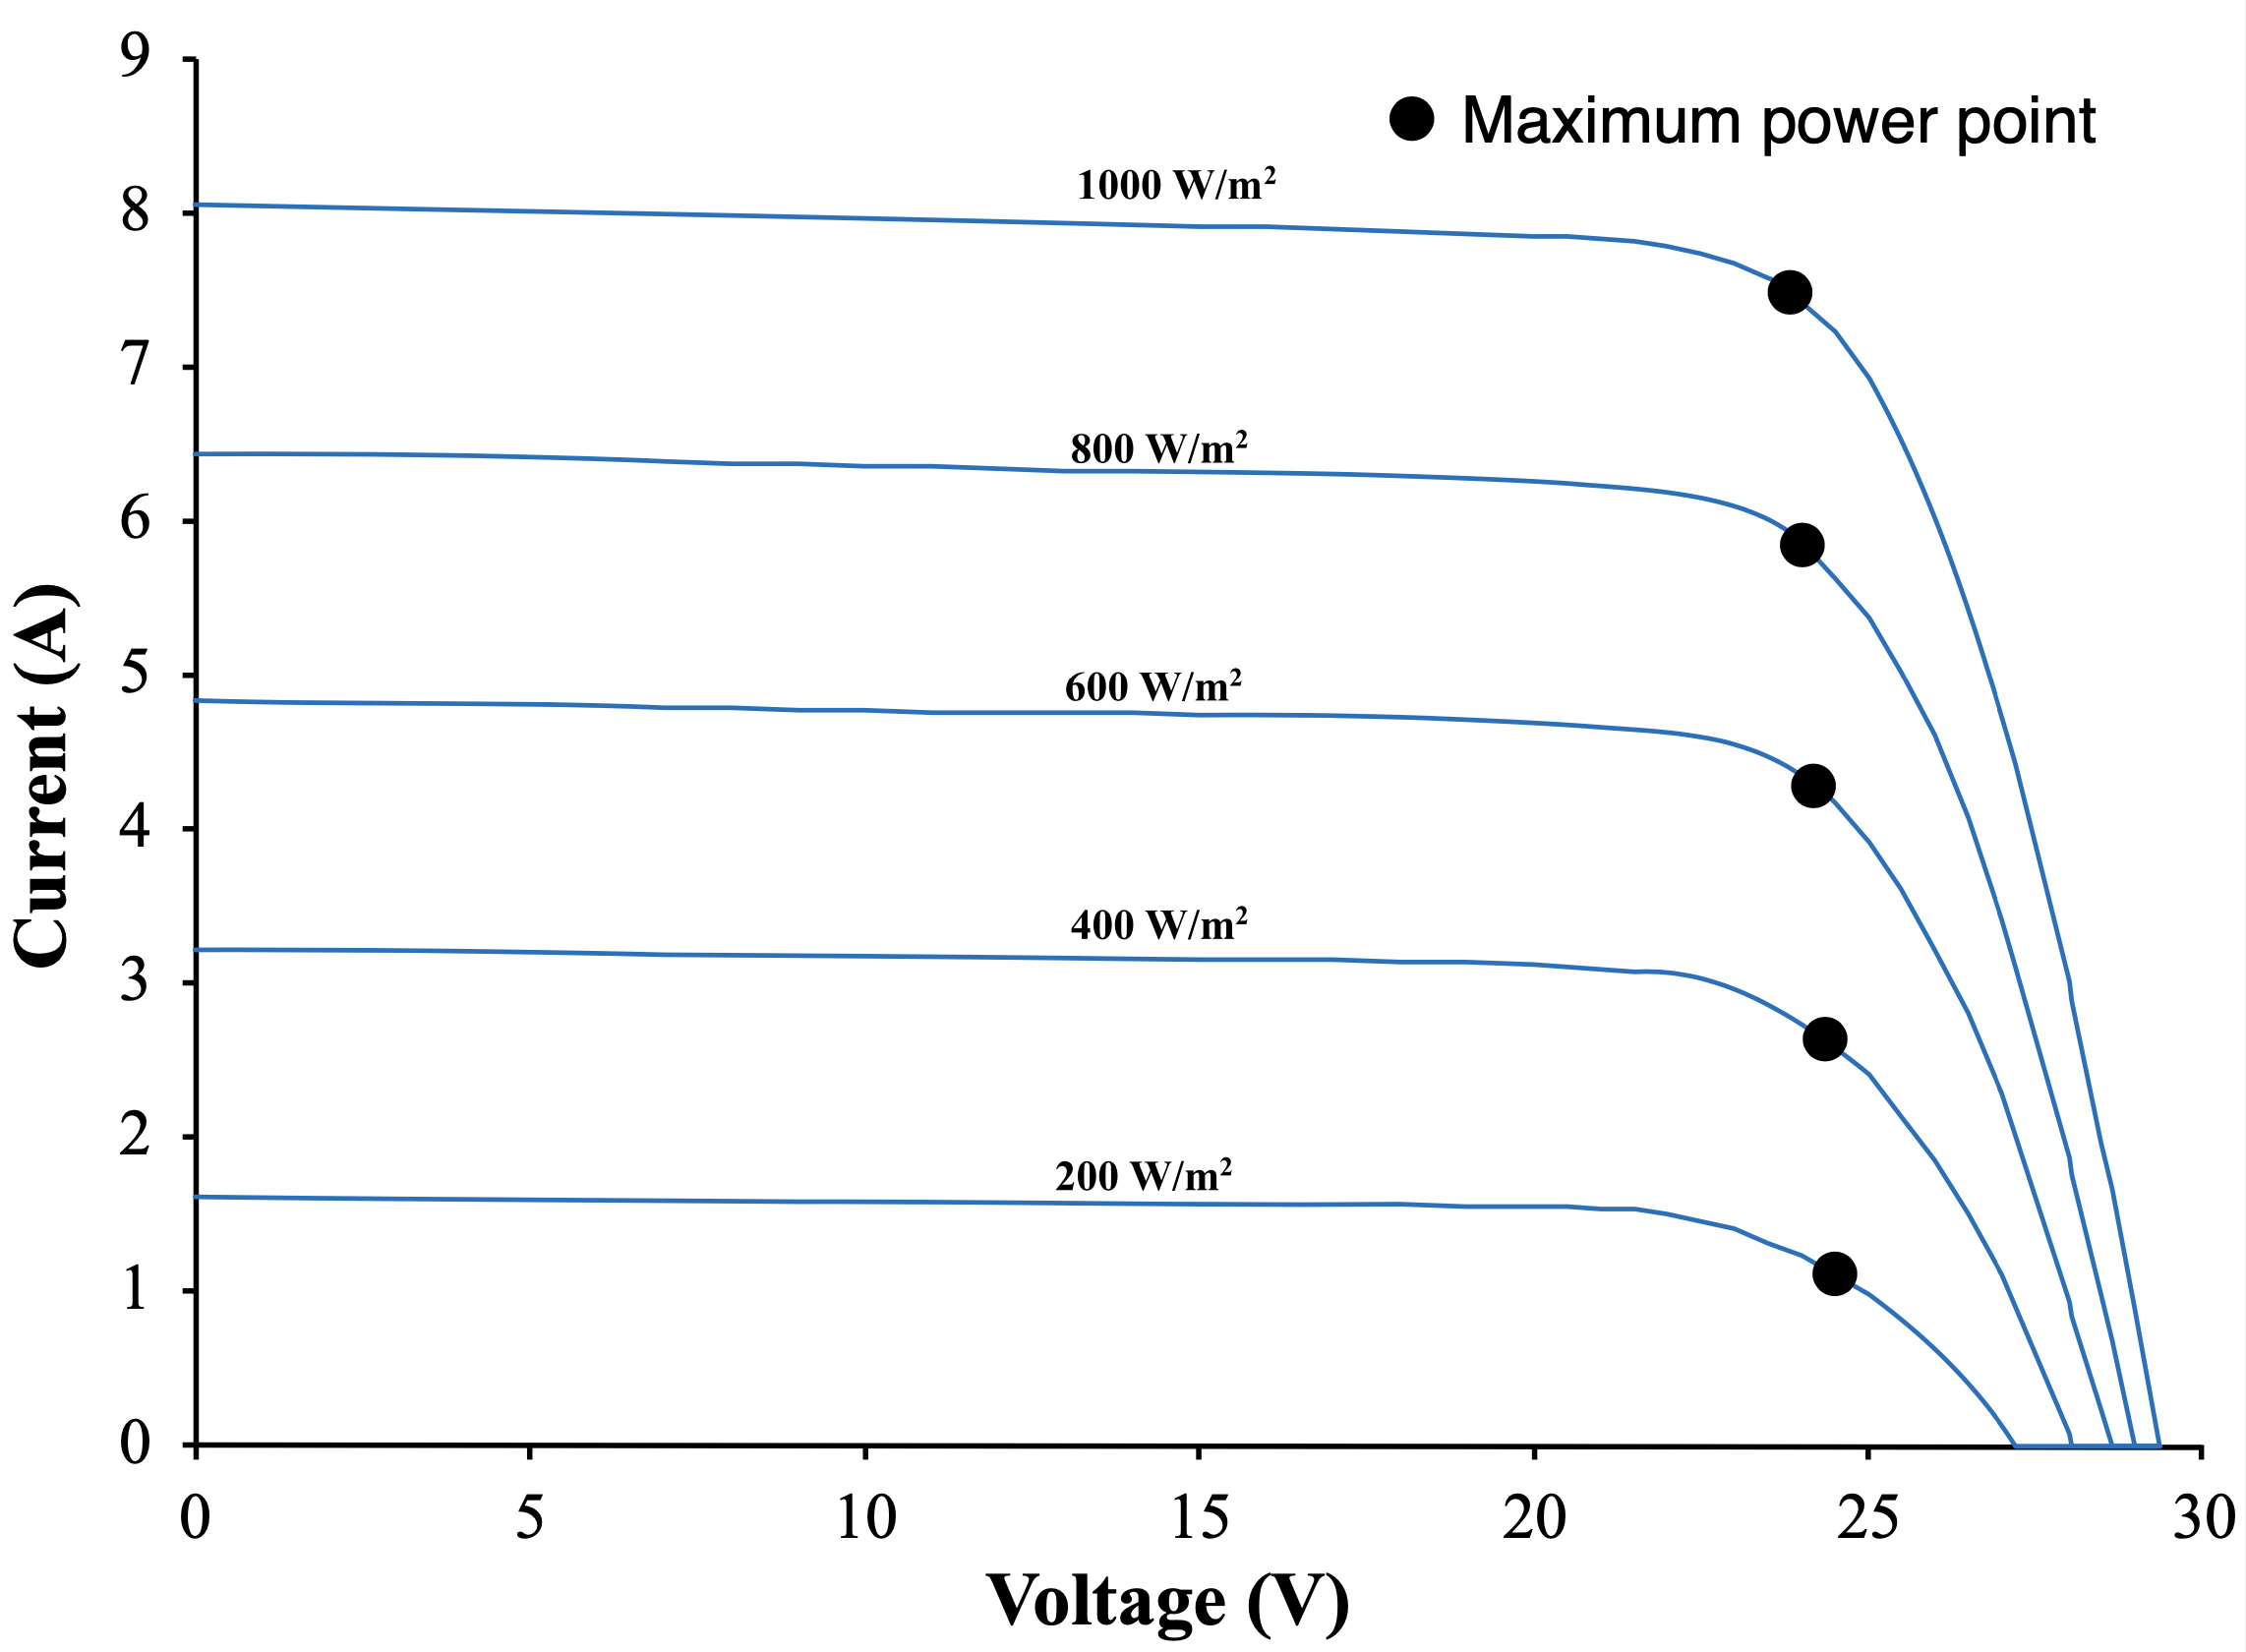
\includegraphics[width=0.9\columnwidth]{ch2_review/figures/solar_iv_pic.png}
    \caption[Typical I-V curves of a PV panel at a constant temperature and different irradiance.]{Typical I-V curves of a PV panel at a constant temperature and different irradiance (adapted from~\cite{ciulla2014comparison}\footnotemark).}
    \label{Figure:solar_vi}
\end{figure}
% This figure is rubbish, can you replace it with a better one if possible!!!!!
\footnotetext{\correct{Reprinted from Renewable and Sustainable Energy Reviews, Volume 32, Ciulla \textit{et al.}, A Comparison of Different One-Diode Models for the Representation of I–V Characteristic of a PV Cell, Pages 684-696, Copyright 2014, with permission from Elsevier.}}

In order to extract as much power as possible out of PV panels, most energy harvesting systems with PV modules adopts maximum power point tracking (MPPT) techniques~\cite{lopez2010new, paz2016high, verma2016maximum}. MPPT is achieved by dynamically controlling the output voltage of PV cells around the MPP.
% When the energy harvester and the energy storage are directly coupled, the operating voltage, which is decided by the charges stored in the energy storage, is usually not at the MPP. However, adopting MPPT circuits inevitably costs energy and reduces the energy efficiency of the whole system. 

Outdoor sunlight and indoor artificial light are two main sources for light energy harvesting. The illumination intensity of direct sunlight on the earth's surface is typically 1000 $W/m^2$~\cite{roundy2004power}, while the typical indoor illumination intensity is 10 $W/m^2$~\cite{shaikh2016energy}. Due to this large difference in the power density of these two circumstances, PV modules are more prospective in outdoor applications for harvesting solar energy. Conversion efficiency of PV cells is typically 15\% to 25\% in outdoor conditions~\cite{mathuna2008energy}.  

Solar energy is an uncontrollable but partially predictable source~\cite{heinemann2006forecasting, buchli2014dynamic}. Solar irradiance demonstrates daily and annual periodicity due to the regularity of celestial movements, as well as irregular variations due to cloud movements, air mass, etc. A 3-year trace of diurnal global horizontal solar energy available measured in Los Angeles from 2012 to 2014 is presented in~\fref{Figure:solar_calendar}, and an example of daily dynamics of global horizontal solar irradiance of the same location is presented in~\fref{Figure:solar_plots}. As shown in both figures, the predictability is reflected from the roughly annual and daily periodicity, and the uncontrollability and randomness relates to the irregular variations, which include both daily variations in an annual scale and variations over a few seconds and minutes on a daily scale. 

\begin{figure}
    \centering
    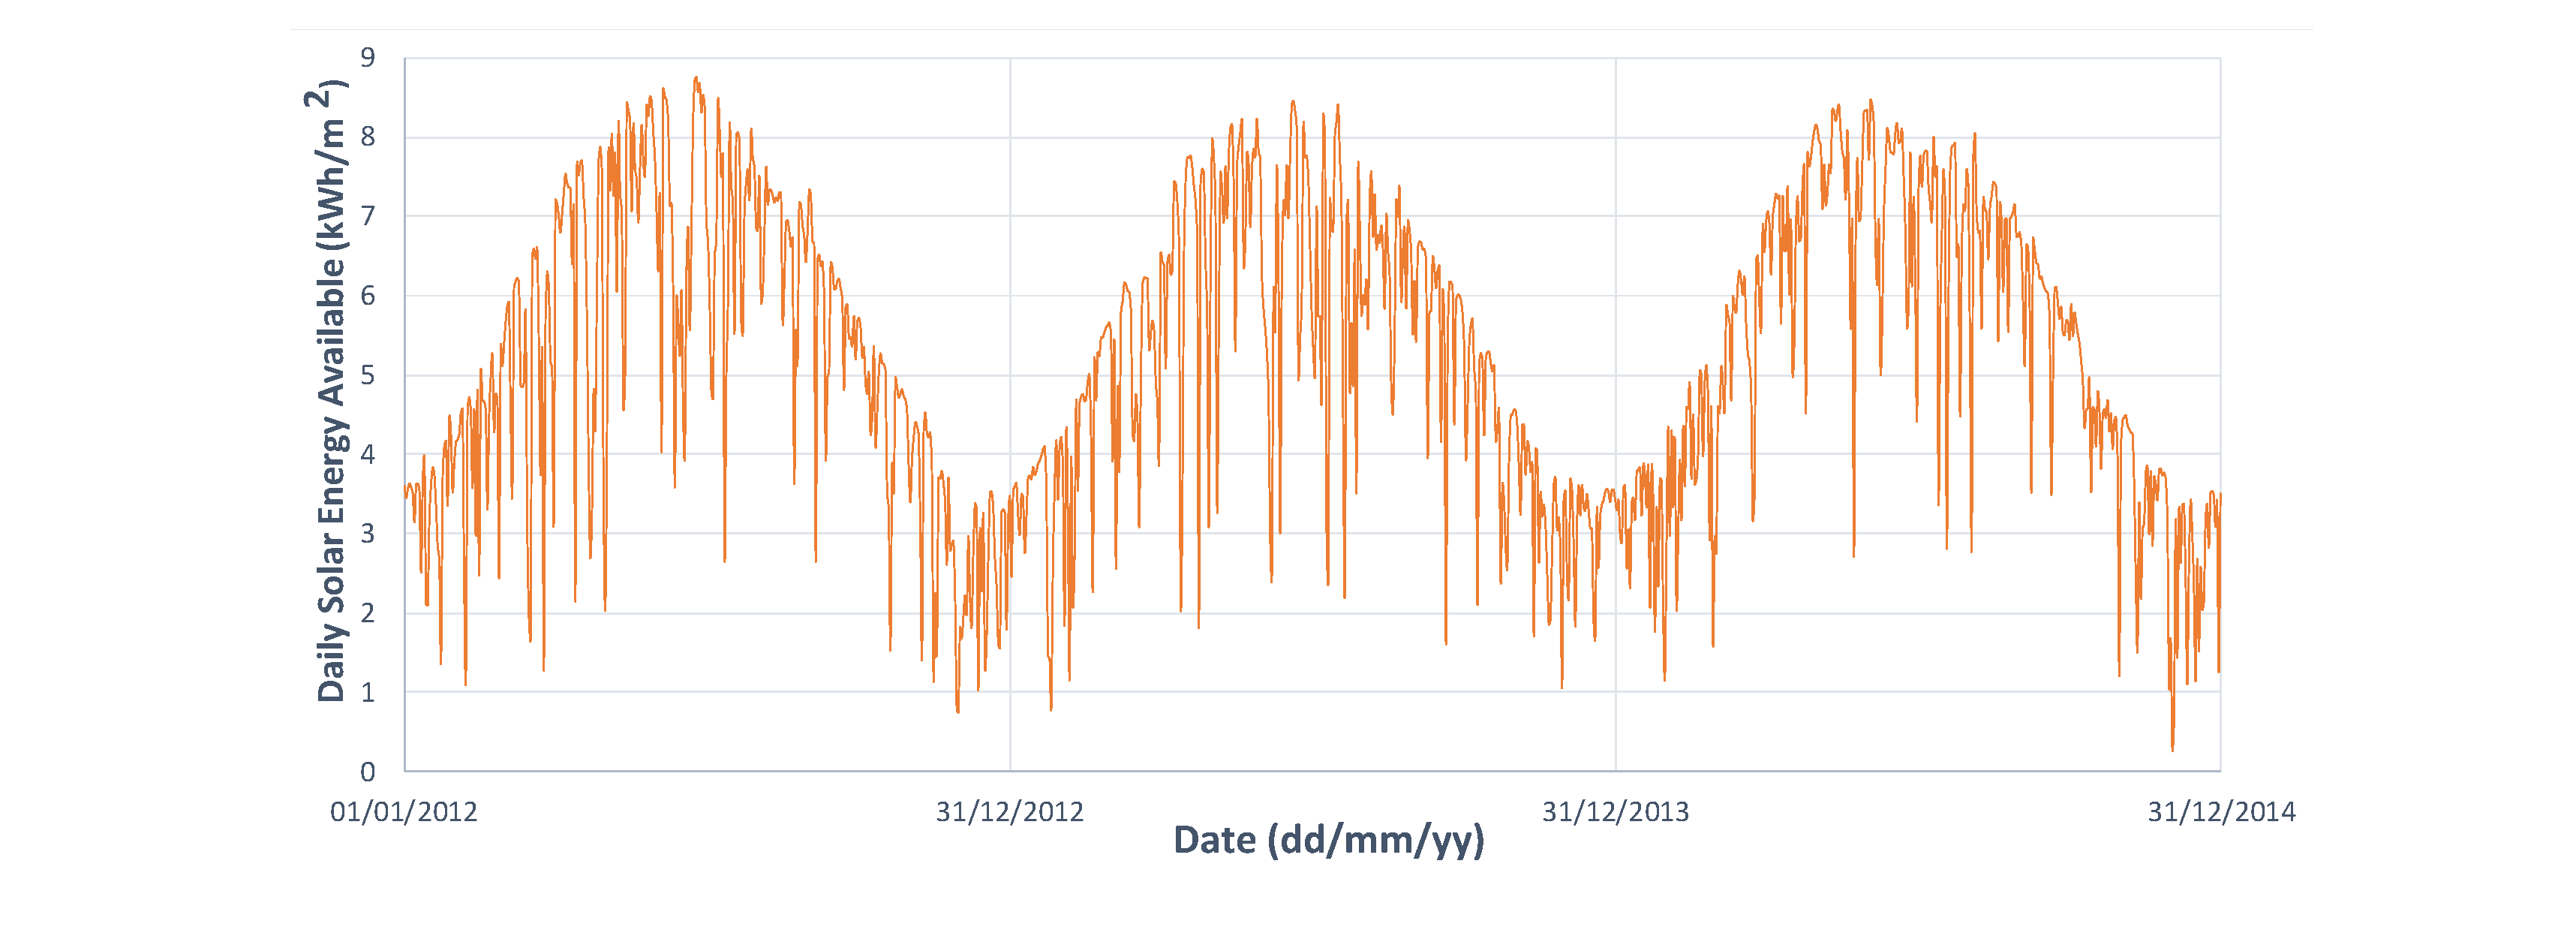
\includegraphics[width=\columnwidth]{ch2_review/figures/solar_calendar}
    \caption{Daily global horizontal solar energy available in Los Angeles 2012-2014~\cite{solar2012}.}
    \label{Figure:solar_calendar}
\end{figure}

\begin{figure}
    \centering
    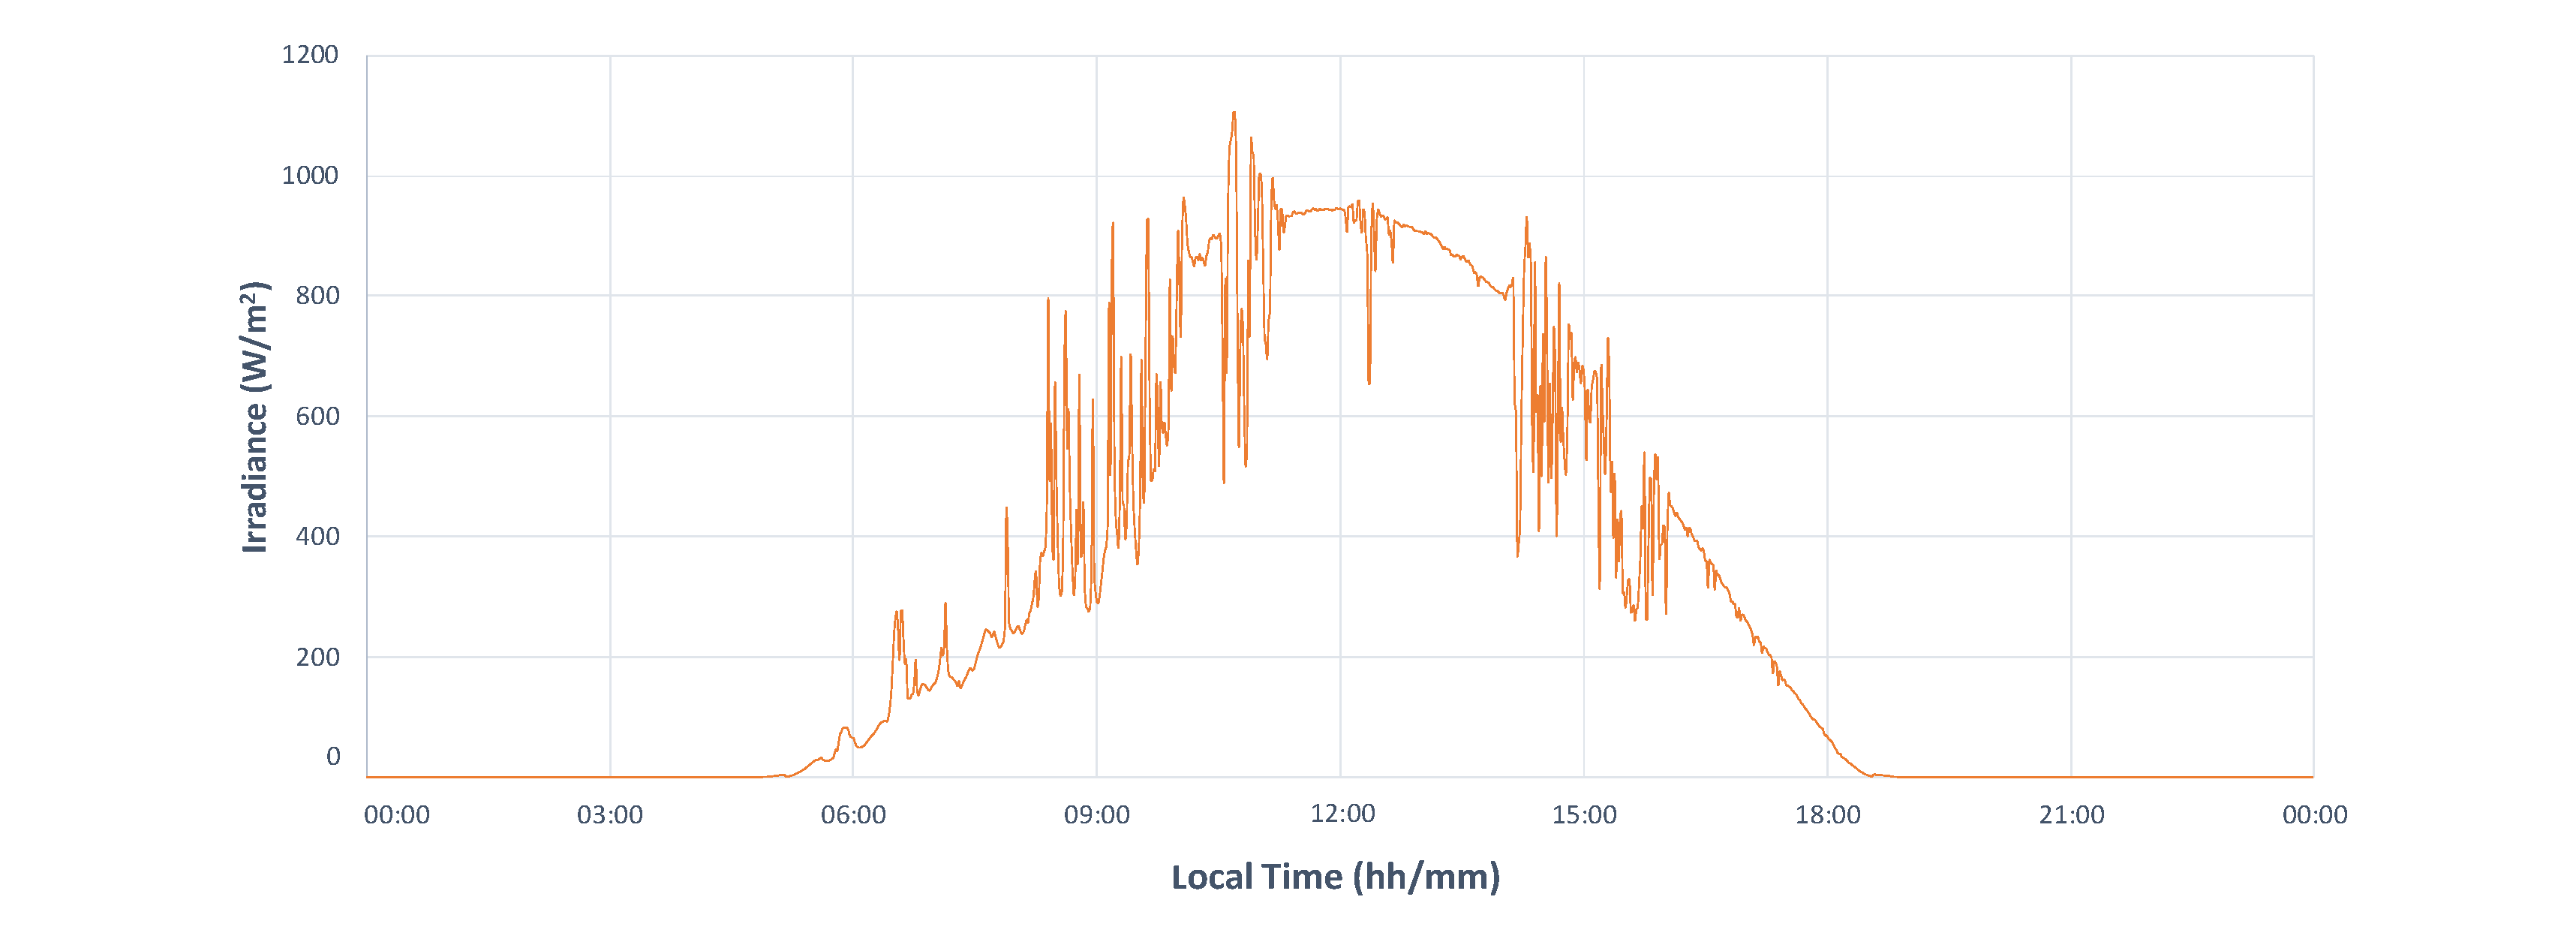
\includegraphics[width=\columnwidth]{ch2_review/figures/solar_plots}
    \caption{One-day dynamics of global horizontal solar irradiance in Los Angeles 29 April 2016~\cite{solar2012}.}
    \label{Figure:solar_plots}
\end{figure}

In order to make full use of solar energy, substantial efforts have been made to develop and improve energy harvesting sensor nodes with solar panels~\cite{raghunathan2005design, seah2009wireless}. Generally, solar energy harvesting approaches adopt large energy storage, e.g. a rechargeable battery, to smooth out the daily and annual variations. Examples of solar-powered sensor nodes are presented in~\cite{raghunathan2005design, corke2007long, kansal2007power}, and a comprehensive review on solar-powered sensor nodes is published in~\cite{sudevalayam2011energy}. 

\subsection{Radio Frequency Energy Harvesting}

Radio Frequency (RF) energy exists in time-varying electromagnetic fields, which widely spread in our environment now due to the propagation of wireless networks, such as Wi-Fi and cellular phone signals~\cite{parks2013wireless}. When radio waves pass through an antenna, due to electromagnetic induction, AC voltage is generated. This AC voltage can be rectified and regulated to DC power for sensor nodes. The received RF power is reciprocal to the square of distance from the source to the destination. The maximum conversion efficiency from RF waves to DC power is typically 50-75\% given a transmission distance of 100 metres~\cite{shaikh2016energy}.
% received power?

Due to the widespread deployment of telecommunication networks, RF energy harvesting becomes available in a wide range of locations, both outdoors and indoors. Compared to light energy harvesting, RF harvesting shows its strength in indoor applications as there is often low or no light intensity inside buildings. 

A basic and common example of RF harvesting is RF Identification (RFID). In a passive RFID application, an RFID reader transmits RF signals to an RFID tag for asking its tag information. The tag absorbs the signals and energy through its antenna, and then responds the reader with its information. Up to now, Wireless Identification and Sensing Platform (WISP)~\cite{sample2008design, naderiparizi2015wispcam} is presented to show the possibility of the integration of RF energy harvesting in IoT applications.

\subsection{Flow Energy Harvesting}

Flow-based energy harvesting utilises turbines and rotors to collect the kinetic energy in air flow or liquid flow. Air flow is converted by wind turbines and liquid flow is converted by hydrogenerators. Wind turbines and hydrogenerators are normally in different mechanical structures (shapes), but the fundamental principles of them are the same.

% Wind turbines are another kind of mature energy harvesters besides PV techniques. 
Wind turbines are manufactured in a wide spectrum in terms of dimensions, from a large-scale wind farm (arrays of large turbines) to a portable micro wind turbine. Micro wind turbines are suitable for battery charging and powering autonomous electronic devices. 

\begin{figure}
    \centering
    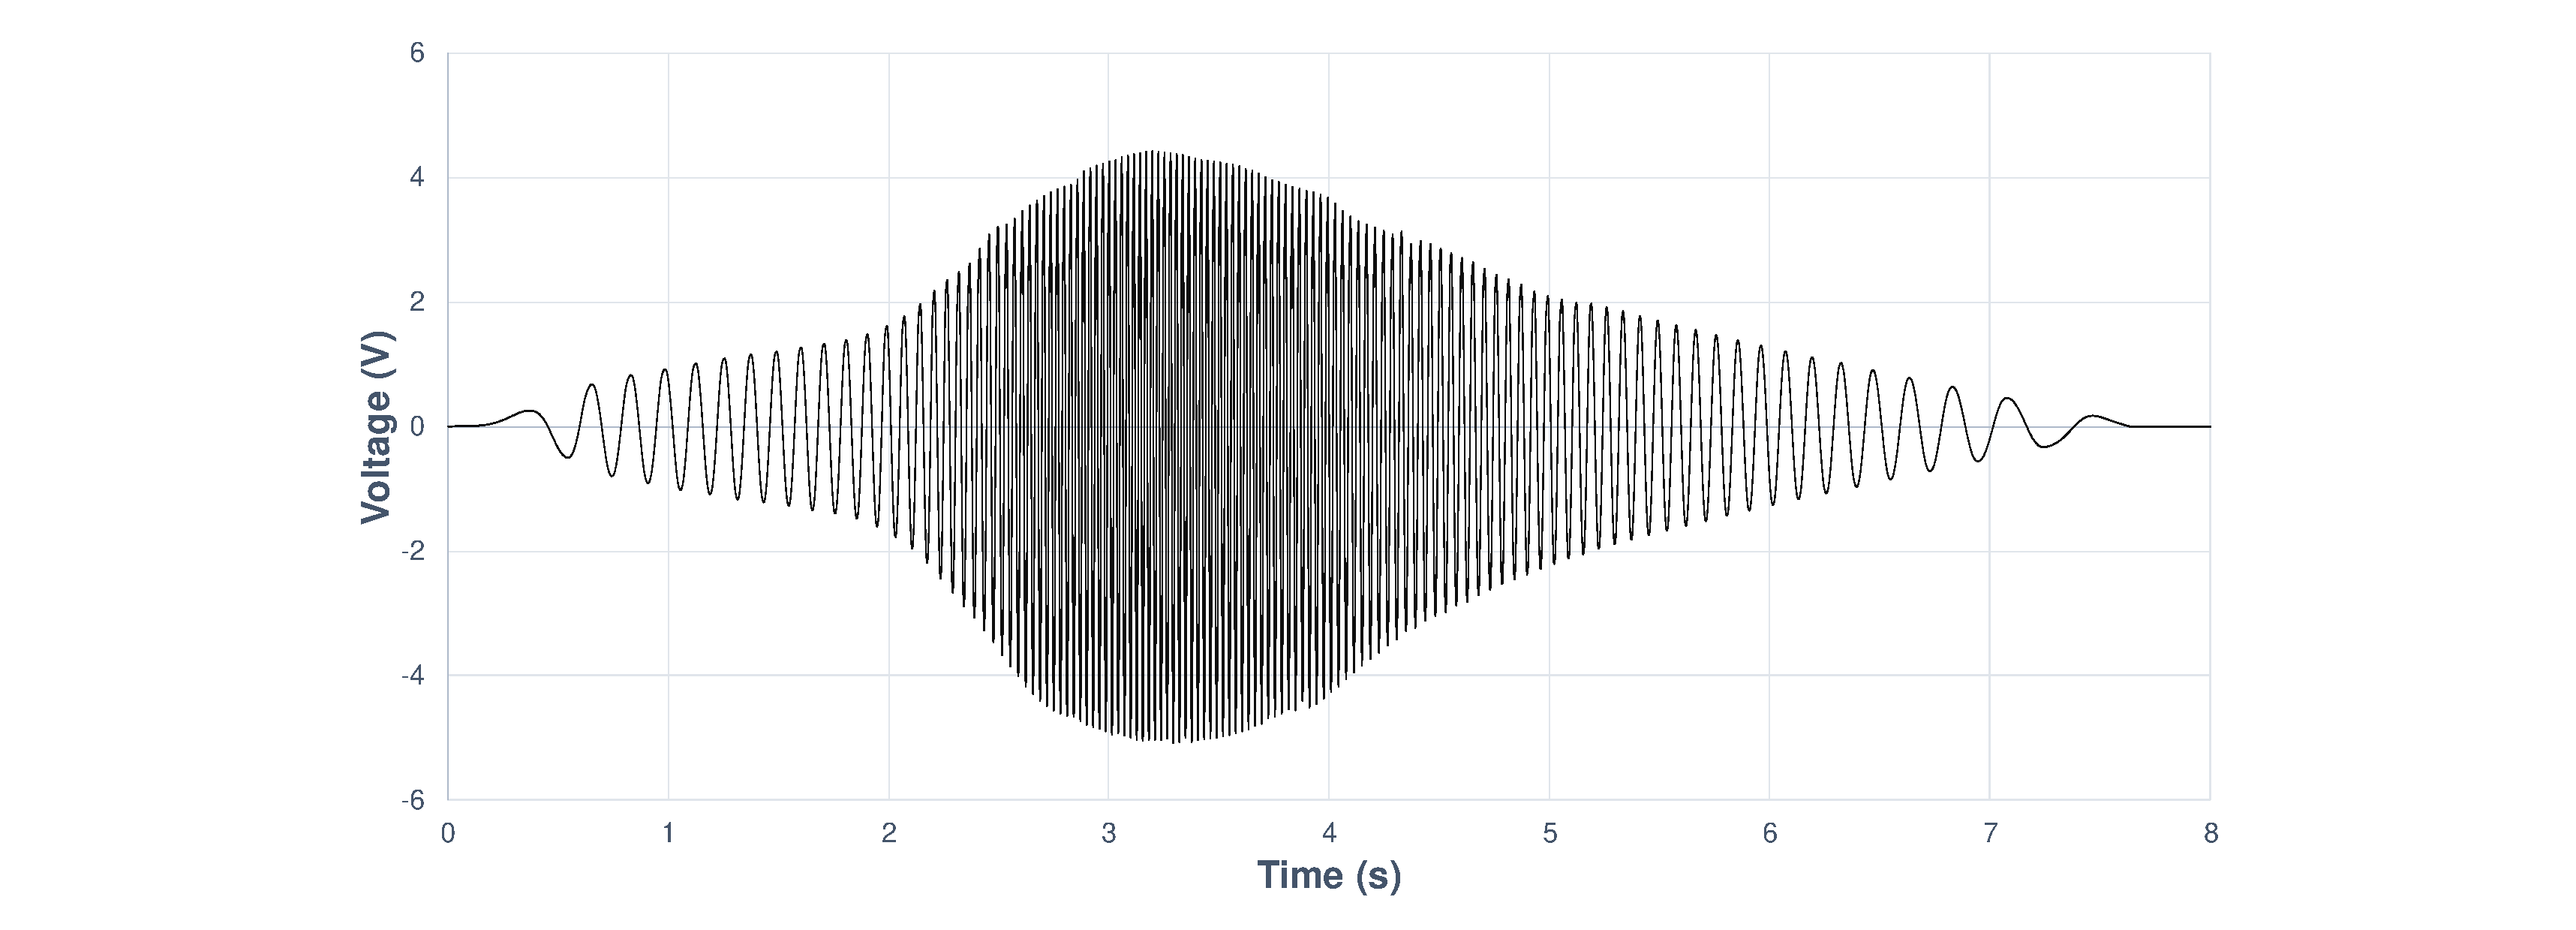
\includegraphics[width=\columnwidth]{ch2_review/figures/micro_wind_turbine}
\caption[Dynamics of a micro wind harvester.]{Dynamics of a micro wind harvester (reproduced from~\cite{balsamo2016graceful}~\correct{© 2016 IEEE}).}
    \label{Figure:micro_wind_turbine}
\end{figure}

A raw voltage output trace of a micro wind turbine given a blast of wind is presented in~\fref{Figure:micro_wind_turbine}. Given a constant blow, a wind turbine should produce a sinusoidal voltage signal. Its voltage output vibrates from the positive domain to the negative domain with time, so a rectifier is normally required in order to utilise this AC power for DC load.

Similar to solar energy, wind energy is uncontrollable but partially predictable. Sharma \textit{et al.}~\cite{sharma2010cloudy} introduce a system that achieves available wind energy predictions based on downloaded weather forecast information within recent 3 days. Also, Cammarano \textit{et al.}~\cite{cammarano2012pro} present a wind and solar energy predicting method which dynamically adjusts its time horizon of prediction in order to achieve higher accuracy than its prior methods. 

Hydrogenerators harness the energy in moving liquids, such as water or a mix of different liquids. Traditionally, hydrogenerators are used for generating large-scale electricity from rivers and streams. However, since the possible underwater applications in IoT, hydrogenerators can be a suitable alternative for powering sensor nodes. For example, Morais \textit{et al.}~\cite{morais2008sun} incorporate a small-sized hydrogenerator as a part of energy harvesting supply for sensor nodes. 

%\fref{Figure:piezo} plots the theoretical rectified power output of a piezoelectric harvester designed in a portable size, as a function of the load resistance $\mathbf{R}$ and the squared coupling coefficient $\mathbf{k^2}$ give a constant external force, where $\mathbf{k^2}$ means the energy conversion efficiency of a piezoelectric material. As observed from \fref{Figure:piezo}, there are one or two optimal loads with the variation of $\mathbf{k^2}$, and with the increase of $\mathbf{k^2}$, the power output approaches a maximum value \cite{shu2006analysis}.

% Mechanical
% \subsection{Mechanical Energy Harvesting}

% Piezoelectricity is the electric effect resulted from the mechanical pressure on certain solid materials, such as lead zirconate titanate (PZT) and polyvinylidene fluoride (PVDF). It is usually used for harvesting vibration and motion energy generated by machines and human walking~\cite{shu2006analysis}. 

% The exemplary power production under certain harvesting conditions is listed in \tref{Table:sources}.

% \begin{table}[!htb]
%     \centering
%     \begin{tabular}{|c|c|c|}
%     \toprule
%     \textbf{Harvester} & \textbf{Energy Source} & \textbf{Harvested Power}\\
%     \midrule
%     Piezoelectric & Footfalls & 1.3mW \cite{shenck2001energy}\\
%     Thermoelectric & Human body heat & 2mW\cite{leonov2013thermoelectric}\\
%     RF & Radio signal & 15.8$\mu$W \cite{parks2013wireless}\\
%     \bottomrule
%     \end{tabular}
%     \caption{Power outputs of various energy harvesters}
%     \label{Table:sources}
% \end{table}

% Thermal Energy
% \subsection{Thermal Energy Harvesting}

% Thermoelectric generators can produce electricity from a temperature difference utilizing the Seebeck effect. This thermal difference can come from human body, industrial devices, geological effects, etc~\cite{beeby2010energy}. 